\section{Scrapbook} \label{sec:Scrapbook}

\subsubsection*{Motivation} This pattern describes a way to make the project meaningful.  

\subsubsection*{Context} We have been working together for a while now.
We have maintained and revised our pattern catalog, and we are
achieving some of the ``What's Next'' steps associated with some of
the patterns.

\subsubsection*{Forces}~
\parbox[t]{.85\textwidth}{
\textbf{Attention}: due to limited energy, we need to ask: where should we set the focus?\\
\textbf{Interest}: new ideas catch our attention\\
\textbf{Meaning}: a history of working on things makes them meaningful.
}

\subsubsection*{Problem} Not all of the ideas we've come up with have proved workable.
Not all of the patterns we've noticed remain equally relevant.
In particular, some patterns no longer lead to concrete next steps.

\subsubsection*{Solution}
In order to maintain focus, is important to ``tune'' and ``prune'' the
things we give our attention to.  We can connect this understanding to
any actions undertaken in the project by asking questions like these:
%%%%%%%%%%%%%%%%%%%%%%%%%%%%%%%%%%%%%%%%%%%%%%%%%%%%%%%%%%%%%%%%%%%%%%%%%%%%%%%%%%%%%%%%%%%%%%%%%%%%
\begin{quote}
(1) Review what was supposed to happen.
(2) Establish what is happening/happened.
(3) Determine what’s right and wrong with what we are doing/have done.
(4) What did we learn or change? 
(5) What else should we change going forward?  \cite[Chapter 28]{peeragogy-handbook}.
\end{quote}
%
%OSS: Who maintains the scrapbook? ... People say when you're learning, you should retain a learning log. Maybe scrapbook is like a shared notebook? All the process should be shared together, even if people take different paths, its all open. Journal of activities?
As current priorities become clearer, we decide where to focus.
Anything that isn't receiving active attention should be moved to a
\patternname{Scrapbook}.  This may encompass:
\begin{itemize}
\item \emph{Retired patterns} whose ``next steps'' have either been
  achieved, set aside, or refactored;
\item \emph{Proto-patterns} made of problems, issues, and concerns
  that have yet to generate concrete next steps;
\item \emph{A back-catalog} of publications, reports, or other
  artifacts that create an institutional memory.
\end{itemize}
In the Peeragogy project, we were initially maintaining a collection
of antipatterns (like `\patternnameext{Magical thinking}') but the
next steps coming from these seemed particularly convoluted and
abstract.  Accordingly, we archived the antipatterns for the time
being.\footnote{\url{http://paragogy.net/Scrapbook}.}  We present a
list of outstanding problems -- without known solutions -- right up
front in the Introduction to the \emph{Peeragogy Handbook}
\cite[Chapter 1]{peeragogy-handbook}.  Our back-catalog includes
academic papers
\cite{building-peeragogy-accelerator,corneli2013inaction,corneli2012paragogical,paragogy-okcon}
and a thesis \cite{corneli-thesis}, earlier editions of the handbook,
as well as informal reports.
%
You don't need to limit
yourself to \emph{your own} creativity: you can include interesting
patterns and ideas from other sources (see \patternname{Reduce, reuse,
recycle}). Ideally many people will contribute by describing their
ideas and concerns, but in some cases a designated
\patternname{Wrapper} may have to do further work to elicit and
organize that material.

\subsubsection*{Rationale} 
We want our pattern catalog to be concretely useful and actively used,
and to keep attention focused on the most relevant issues.
If a pattern is not specifically useful or actionable at the
moment, sufficient time for reflection may offer a better
understanding, or it may prove useful in a different context.

\subsubsection*{Resolution} 
Judicious use of the \patternname{Scrapbook} can help focus project participants' \textbf{attention} on current concerns, without losing grasp of items of \textbf{interest}.  The currently active pattern catalog is leaner and more action-oriented as a result. If the \patternname{Roadmap} shows where we're going, it is the \patternname{Scrapbook} that shows most clearly where we've been, and collects the observations that are most \textbf{meaningful} to us.

\begin{wrapfigure}{r}{.52\textwidth}
\vspace{-1.9cm}
\begin{center}
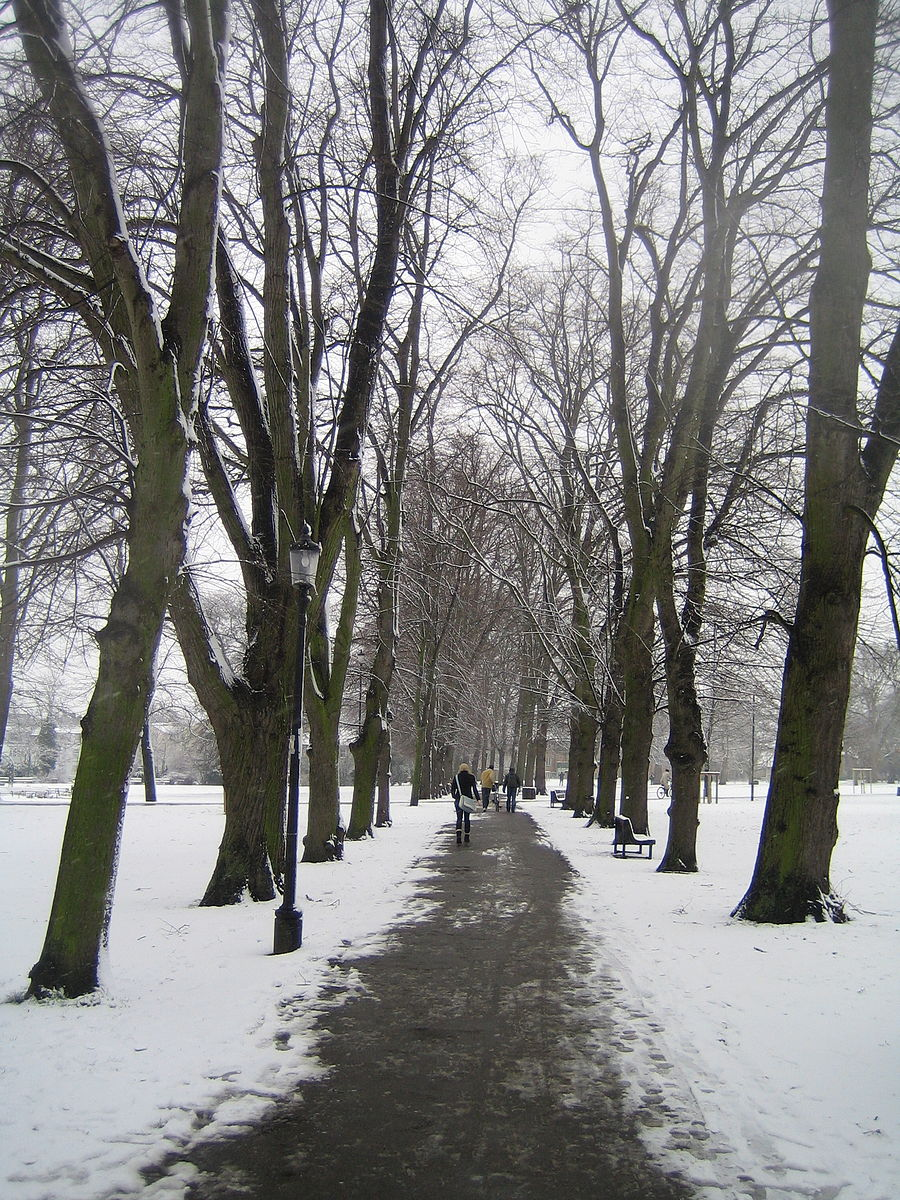
\includegraphics[width=.5\textwidth,trim=0 200 0 0, clip=true]{ChristsPieces}
\end{center}
\vspace{-.5cm}
\caption{Christ's Pieces, Cambridge, UK. Public
  domain.\label{christs-pieces}}
\vspace{-1.7cm}
\end{wrapfigure}

\subsubsection*{Example 1} The history of the Wikimedia Foundation,
and of Wiki\-pedia, are maintained as wiki
pages.\footnote{\url{https://wikimediafoundation.org/wiki/History_of_the_Wikimedia_Foundation}}\textsuperscript{,}\footnote{\url{https://en.wikipedia.org/wiki/Wikipedia}}
There is also a page on Wikipedia detailing
critiques.\footnote{\url{https://en.wikipedia.org/wiki/Criticism_of_Wikipedia}}
Five years on, the previous ``five year plan'' somewhat resembles a \patternname{Scrapbook} \cite{wikimedia2011plan}.  

\subsubsection*{Example 2} 
In the future university, the patterns described here will continue to
shape the landscape, but considerable activity will be focused on new
problems and new patterns -- just as a university campus grows and
changes in an emergent fashion over time.


\begin{framed}
\noindent 
\emph{What's Next in the Peeragogy Project}
\definecollection{ScrapbookWN}
\begin{collectinmacro}{\ScrapbookWN}{}{}
After pruning back our pattern catalog, we want it to grow again: new patterns are needed.
One strategy would be to ``patternize'' the rest of the \emph{Peeragogy Handbook.}
\end{collectinmacro}
\ScrapbookWN
\end{framed}


\newpage
